%!TEX root = ../thesis.tex
%*******************************************************************************
%*********************************** First Chapter *****************************
%*******************************************************************************

\chapter{Consistency}  %Title of the First Chapter

\ifpdf
    \graphicspath{{Chapter10/Figs/Raster/}{Chapter10/Figs/PDF/}{Chapter10/Figs/}}
\else
    \graphicspath{{Chapter10/Figs/Vector/}{Chapter10/Figs/}}
\fi

\label{chapter 10}


%************************************************************************** 

A reflective Dirichlet boundary condition is validated for perfect conducting wall in rotated Brio-Wu test in chapter \ref{chapter 4}, based on Dirichlet boundary condition suggested by Sambasivan and UdayKumar \cite{sambasivan2009ghost}. The resistive boundary condition represented by equation \ref{equ:magneticDiffusion} is applied in cylindrical equilibrium in chapter \ref{chapter 8}, similar to most of resistive wall relevant papers \cite{chrysanthou2020,ferraro2016multi,becerra2016resistive,hender1989effects}. These methods are all mainstream methods. Yet, it seems that when the resistivity approaches zero, it's still quite different from when the resistivity is exactly zero, as shown in Figure \ref{fig:totalEnergy}. In this chapter, we are going to analyze superconducting wall condition and extend these into a general wall condition, which may help to address this inconsistency.

\section{Superconducting Wall Condition}
\subsection{London Equations and Meissner Effect}
We start from some basic theories of London Equations. London Equations are relevant to Meissner effect in superconductors \cite{london_equations_wikipedia}. The Meissner effect is the phenomenon where a superconductor expels magnetic fields from its interior when it transitions into the superconducting state. We focus on the London equations and the reasoning behind their derivation.

It starts from the definition of current density. The current density is defined as 
$$
\mathbf{J}_s=-n_s q_e \mathbf{v}_s\ ,
$$
Where the $q_e$ is the elementary charge on a single electron with  $q_e=-1.602176634\times10^{-19}$, a negative number. The $n_s$ and $\mathbf{v}_s$, in simple terms, are electron number density and velocity, where lower index $s$ specify a superconductor situation. We have the Newton's Second Law of Motion for electron
\begin{equation}
m\frac{d\mathbf{v}_s}{dt}=-q_e\mathbf{E}\ ,
\label{equ:motion_perfectConducting}
\end{equation}
where $m$ is the electron mass and $\mathbf{E}$ is the electric field. By getting the time derivative of current density $\mathbf{J}_s$ and substituting velocity derivative over time with equation \ref{equ:motion_perfectConducting}, it gives the London First Equation
$$
\frac{\partial \mathbf{J}_s}{\partial t}=\frac{n_s q_e^2}{m}\mathbf{E}\ .
$$
This describe the relationship in a superconductor, electric field accelerate electrons and increase the current density. By taking a curl on both sides and substituting the $\nabla\times\mathbf{E}=-\frac{\partial \mathbf{B}}{\partial t}$ with Faraday's law, it gives
$$
\frac{\partial }{\partial t}\left(\nabla\times\mathbf{J}_s+\frac{n_s q_e^2}{m}\mathbf{B}\right)=0\ .
$$

From the Meissner effect, it is found that $\mathbf{B}=0$ holds for all superconductor and $\nabla\times\mathbf{J}_s$ can not be a non-zero constant. It gives the London Second Equation
$$
\nabla\times\mathbf{J}_s+\frac{n_s q_e^2}{m}\mathbf{B}=0\ .
$$
Further replacing current density by static condition of Ampere's Law, $\mathbf{J}_s=\nabla \times \mathbf{B}$, this give a equation that only contain magnetic field. Along with identity $\nabla\times\nabla\times\mathbf{B}=\nabla\left(\nabla\cdot\mathbf{B}\right)-\nabla^2\mathbf{B}$, while $\nabla\cdot\mathbf{B}=0$, these give \cite{london_equations_wikipedia} 
\begin{equation}
	\nabla^2\mathbf{B}=\frac{1}{\lambda_s^2}\mathbf{B}\ ,\ \ \ \ \ \  \lambda_s^2=\frac{m}{n_s q_e^2}\ .
	\label{equ:B_superconducting}
\end{equation}


\subsection{Penetration on Superconductor Wall}
This equation \ref{equ:B_superconducting} give us some information on magnetic field within superconductors. If we place a magnetic field, we may know about the strength distribution and how the superconducting wall reflect the normal component of magnetic field. We place a wall in vacuum. As depicted in Plot \ref{fig:magneticPenetration}, a normal magnetic $\mathbf{B}=B_0\mathbf{i}$ is imposed on the wall suddenly. The x dimension is the only mattering direction. This give a equation along x.
\begin{equation}
	\frac{\partial^2 B_x}{\partial x^2}=\frac{1}{\lambda_s^2}B_x\ .
\end{equation}
It is a homogeneous second order differential equation, a Helmholtz equation \cite{london_equations_wikipedia}. A general solution can be given as $B_x(x)=C_1e^{\frac{x}{\lambda_s}}+C_2e^{-\frac{x}{\lambda_s}}$. Some physical boundary conditions are given as $B_x(0)=B_0$ and $\lim_{x \to \infty} B_x(x)=0$. These define the solution
\begin{equation}
	B_x(x)=B_0e^{-\frac{x}{\lambda_s}}\ .
\end{equation}
$\lambda_s$ is 'penetration depth' controlling the penetration. Even for superconductors, there will be some penetration. As discussed in chapter \ref{chapter 6}, the superconducting materials used in ITER and EAST are Nb3Sn and NbTi. Their penetration depths are around $\lambda_{Nb3Sn}=8.0\times10^{-8}m$ and $\lambda_{NbTi}=1.0\times10^{-7}m$. For a better visualization, we add a simple case    $\lambda_{0}=4.6\times10^{-4}m$ based on the relevant parameter on tungsten \cite{greiner2012classical}. Their penetrations under simply $B_0=1.0$ are demonstrated in Figure \ref{fig:PenetrationCurveSuperconducting}. After penetrating into a superconducting wall, the magnetic field is fully countered off. This form a 'no-penetration' condition on normal magnetic field. A reflective boundary is applied on this condition. We proved these mathematically in chapter \ref{chapter 2}. 
 
\begin{figure}[H]
	\centering
	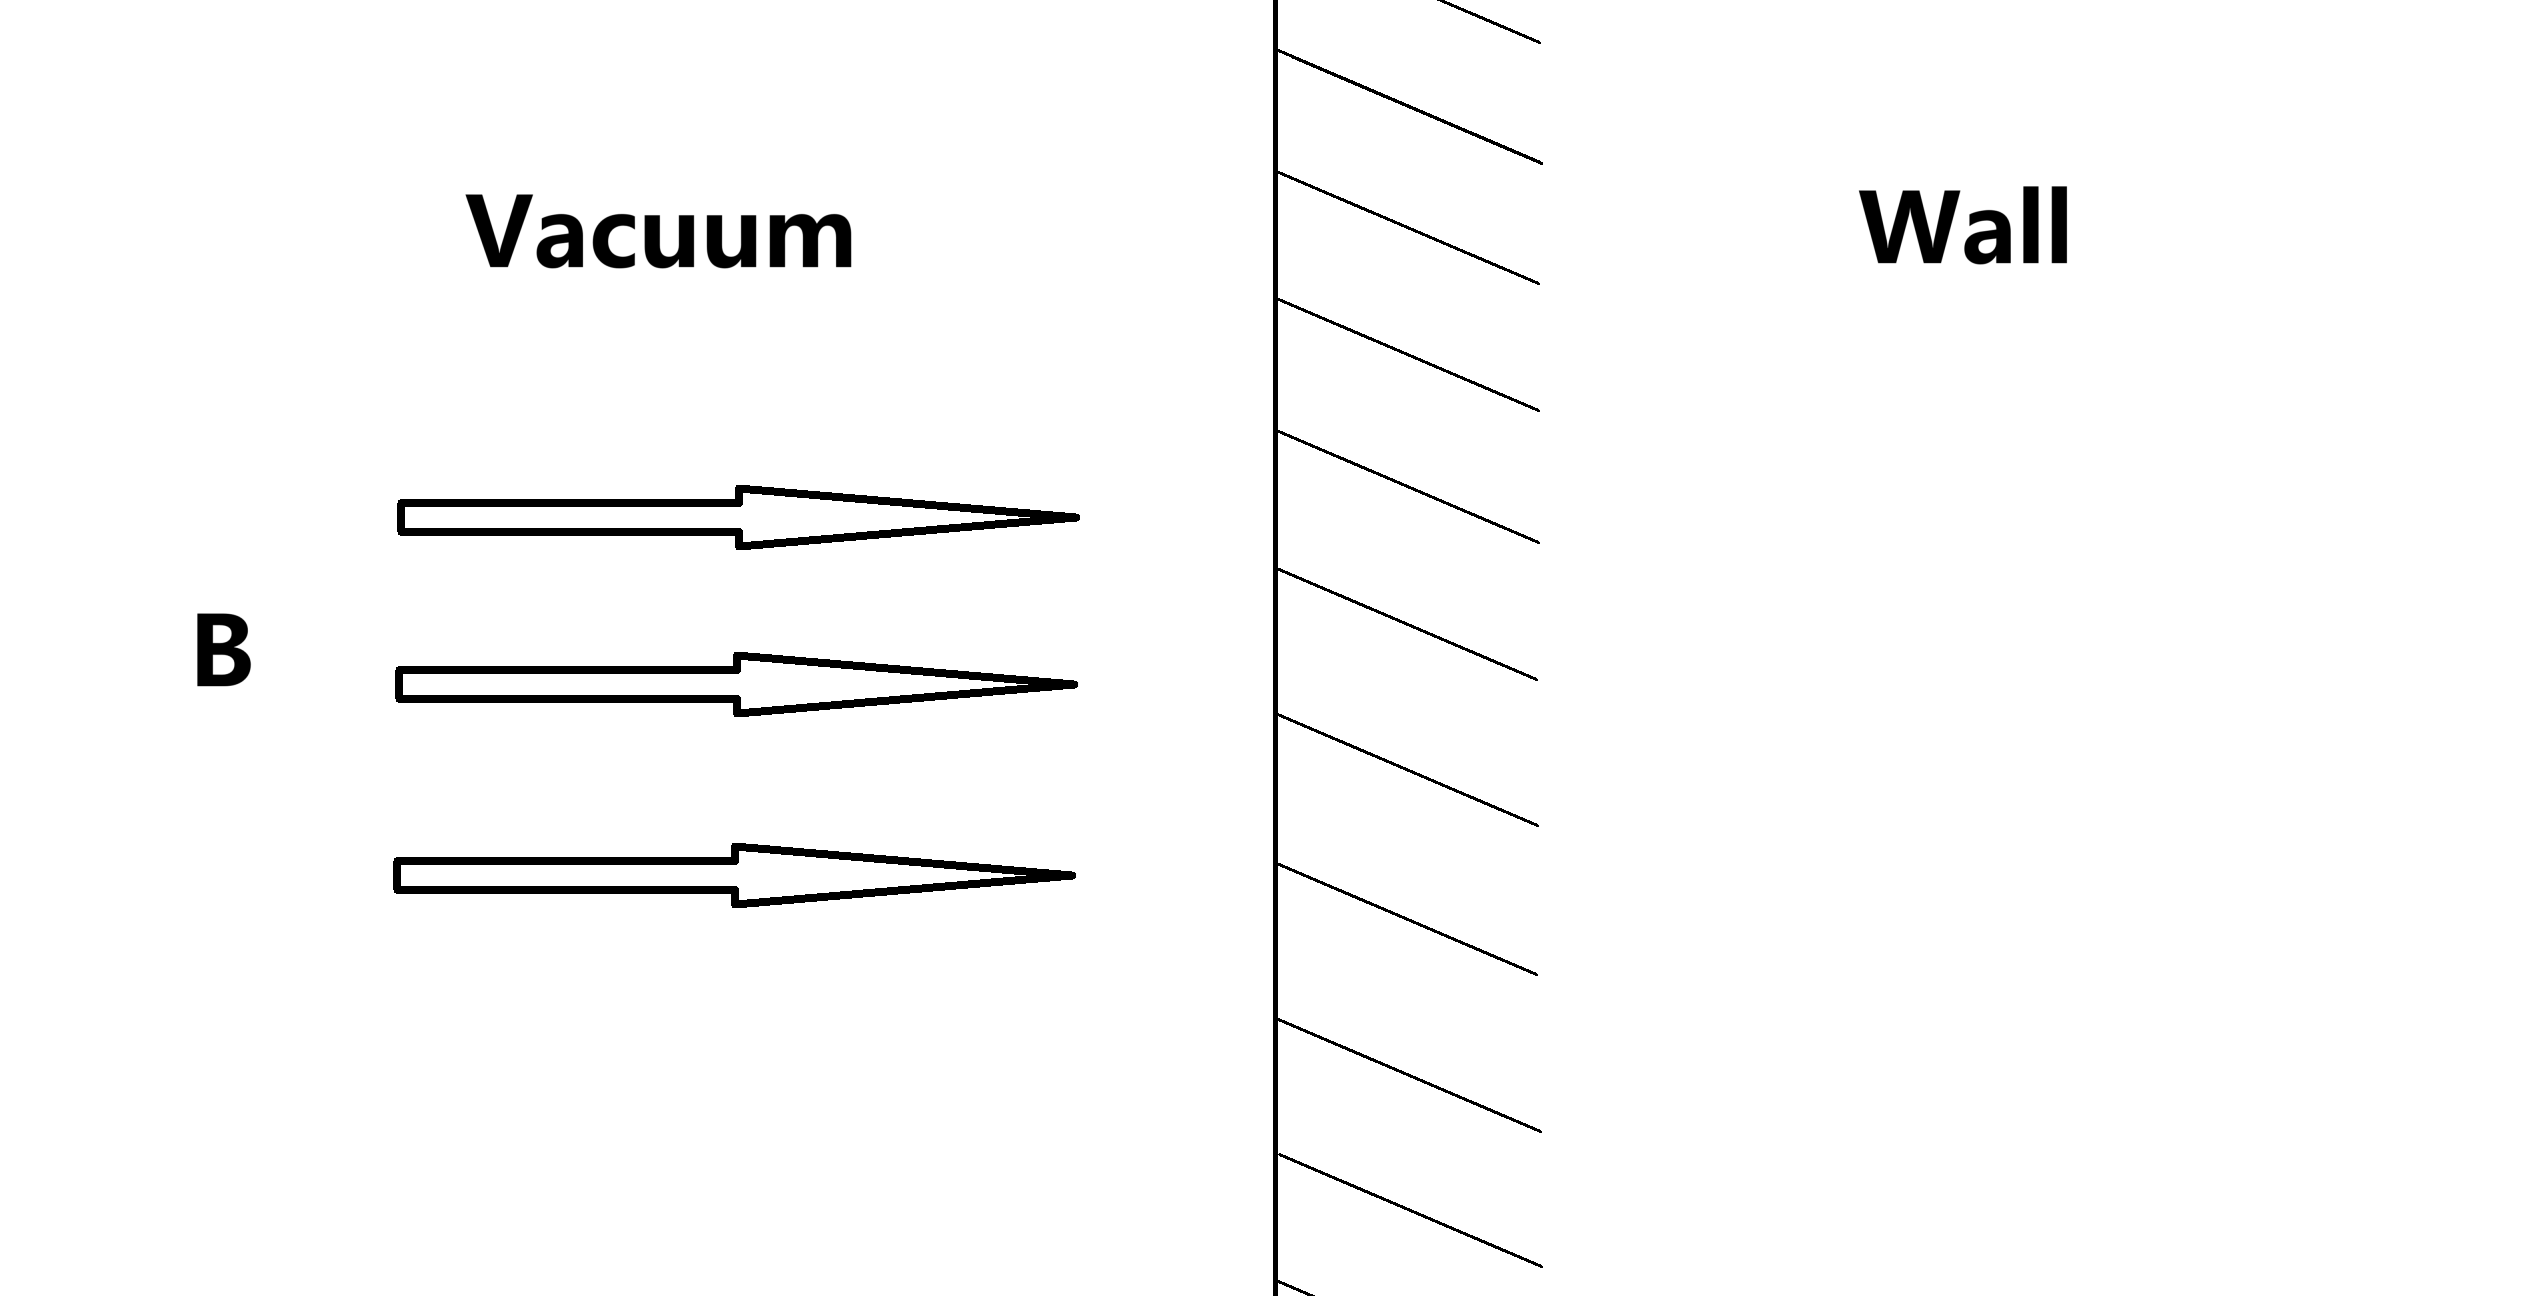
\includegraphics[width=0.8\linewidth]{BPenetration.png}
	\caption[Magnetic Penetration]{An illustration of normal magnetic field on a conducting wall. The entire space is divided into two parts: the left side ($x<0$) is a vacuum, and the right side ($x\geq0$) is a wall made of a certain conductor material. A homogeneous normal magnetic field $\mathbf{B}=B_0\mathbf{i}$ is suddenly imposed on the wall. The extent to which the magnetic field penetrates the wall depends on the resistivity of the wall's material.}
	\label{fig:magneticPenetration}
\end{figure}

\begin{figure}[H]
	\centering
	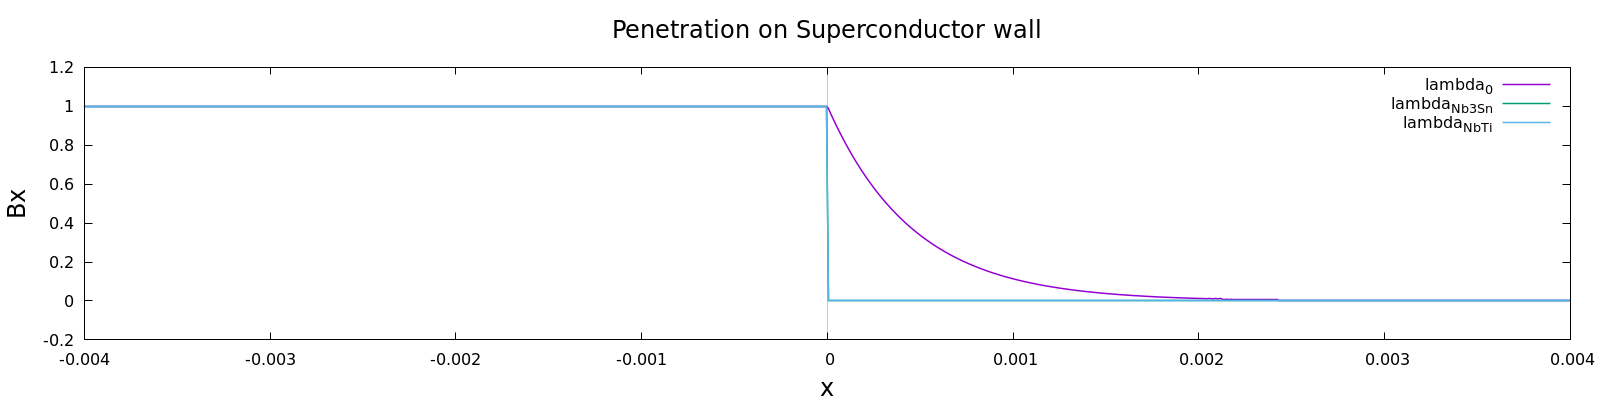
\includegraphics[width=1\linewidth]{penetration_superconducting.png}
	\caption[Bx Distribution]{Magnetic penetration along x.}
	\label{fig:PenetrationCurveSuperconducting}
\end{figure}

\section{Extension on General Wall}
We make an extension into a general wall condition. A similar relationship still hold for current density based on free number density $n$,  
$$
\mathbf{J}=-n q_e \mathbf{v}\ .
$$
However, in the Newton's Second Law of Motion, we need to consider the effect of resistivity. In microscopic point of view, electron collides when moving along conductor. We use collision frequency $\nu$ to represent such phenomenon. The resistivity $\eta_w$ and $\nu$ have relation $\eta_w=\frac{nq_e^2}{\nu m}$. In Kittle \cite{kittel2018introduction}, a similar collision time $\tau$ and conductivity are defined. From a macroscopic perspective, this behaves like damping \cite{kittel2018introduction}. The motion of electron can be given by 
$$
m\frac{d\mathbf{v}}{dt}+m\nu \mathbf{v}=-q_eE\ .
$$

Solving this differential equation for $\mathbf{v}$ along with a initial condition $\mathbf{v}_0=0$, give the solution 
$$
\mathbf{v}=-\frac{q_e\mathbf{E}}{\nu m}+\frac{q_e\mathbf{E}}{\nu m}e^{-\nu t}\ .
$$

After taking curl and applying the Faraday's Law, we rearrange the equation and substitute some terms with $\eta_w$. These give the equation
\begin{equation}
	\nabla^2\mathbf{B}=\frac{nq_e^2}{m\nu}\frac{\partial \mathbf{B}}{\partial t}-\frac{nq_e^2}{m\nu}e^{-\nu t}\frac{\partial \mathbf{B}}{\partial t}
\end{equation}

\section{Boundary Condition Recap} 
This equation gives a more consistent resistive boundary condition rather than equation \ref{equ:magneticDiffusion}.
\subsection*{Perfect Conducting Wall}
For perfect conducting wall, L'Hopital's Rule gives $$
\lim_{\nu \to 0}\frac{1-e^{-\nu t}}{\nu}=\frac{\frac{\partial(1-e^{-\nu t})}{\partial t}}{\frac{\partial\nu}{\partial t}}=-t\ .
$$ 
With a perturbation method applied, the change over time is small and approximately linear $t\frac{\partial \mathbf{B}}{\partial t}\approx\mathbf{B}$. It gives 
$$
\nabla^2\mathbf{B}=\frac{n q_e^2}{m}\mathbf{B}\ .
$$
This is the same as discussed in superconducting case. We have shown that a reflective Dirichlet boundary condition is appropriate in this case.

\subsection*{Resistive Wall and Insulator Wall}
For a resistive wall, $\nu$ is big and $e^{-\nu t}$ can be ignored. With relation $\eta_w=\frac{nq_e^2}{\nu m}$, we have 
$$
\eta_{w}\nabla^2\mathbf{B}=\frac{\partial \mathbf{B}}{\partial t}\ .
$$
This is exactly the case we use in resistive wall in equation \ref{equ:magneticDiffusion_rearrange}. We deal with this boundary condition by updating it using some similar ghost fluid methods. These give results in earlier chapters. Insulator wall is just an extreme case of this situation. It is more convenient to just set it to be Neumann.

\subsection*{Small Resistivity}
In the Plot \ref{fig:totalEnergy}, the inconsistency happens when 
$$
\lim_{\nu \to 0,\eta_w \to 0}\ Resistive\ Wall \neq Perfect\ Conducting\ Wall\ .
$$
This equation enable us to know more about the situation when resistivity get close to 0 but not 0. We have series expansion of $e^{-\nu t}=\sum_{n=0}^{\infty}\frac{1}{n!}\nu^nt^n$. With the assumption that magnetic field change slightly over time and $\nu$ is small, t$\frac{\partial \mathbf{B}e^{-\nu t}}{\partial t}\approx\mathbf{B}e^{-\nu t}$. These give the equation 
\begin{equation*}
	\nabla^2\mathbf{B}=\frac{e^{-\nu t}}{\lambda^2}\mathbf{B}\ ,\ \ \ \ \ \  \lambda^2=\frac{m}{n q_e^2}\ .
\end{equation*}
A solution on x coordinate is
\begin{equation}
	B_x(x)=B_0e^{-\frac{xe^{-\frac{\nu t}{2}}}{\lambda}}\ .
\end{equation}

Figure \ref{fig:smallResistivityWall} demonstrate some visualization of this solution. For simplicity, we use $\nu=1.0$ and $\lambda_{0}=4.6\times10^{-4}m$. It seems that when the normal magnetic component impose on the small resistive wall, it react like a perfect conducting wall as in superconducting situation. The only effect of resistivity is to gradually allow the magnetic field to penetrate the wall over time. Based on the numerical methods we have, it seems that using a reflective boundary condition for the plasma while updating the rigid body magnetic field provides a better approximation for the boundary case with small resistivity.  

\begin{figure}[H]
	\centering
	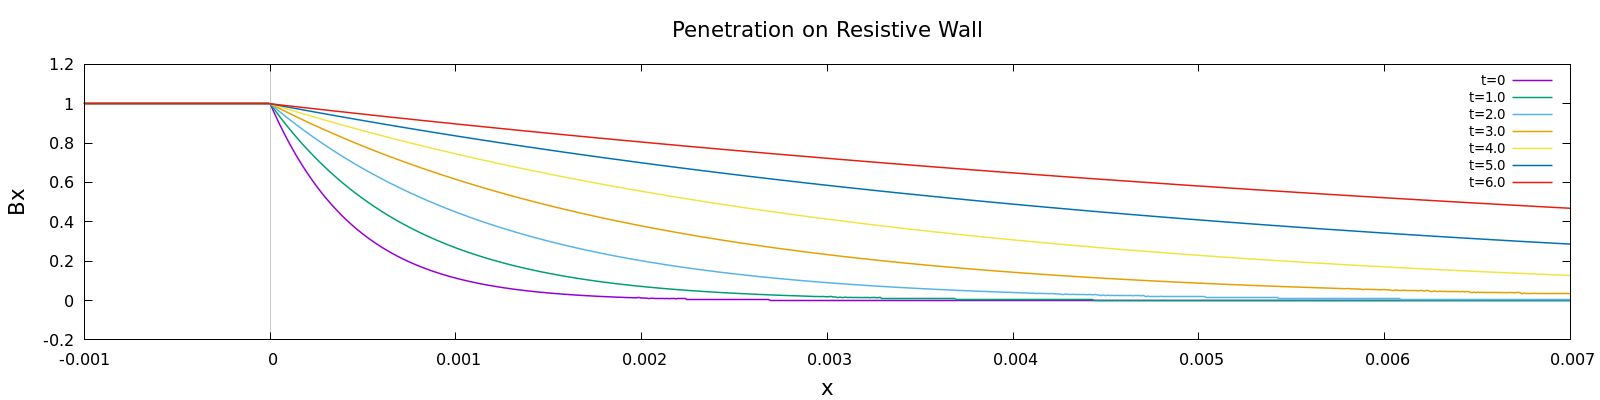
\includegraphics[width=1\linewidth]{penetration_wall.png}
	\caption[Bx distribution on resistive wall]{Magnetic distribution on a resistive wall. When a normal magnetic field is applied to a small resistive wall, the initial magnetic field distribution inside behaves as if it were in a perfect conductor. However, the resistivity causes the magnetic field to slowly penetrate the wall over time.}
	\label{fig:smallResistivityWall}
\end{figure}
\section{Addressing the Inconsistency}
Generally, the inconsistency happens when $\lim_{\eta_w \to 0}$. This is because we only consider a damping effect on electrons when $\eta_w>0$ in Maxwell's equation of $\eta_w\mathbf{J}=\mathbf{E}$. However, for $\eta_w=0$, acceleration is the only factor considered. For example, in London Equations $m\frac{d\mathbf{v}_s}{dt}=-q_e\mathbf{E}$, where the electric field accelerates electrons infinitely. Hence, inconsistency occurs when neither of these effects can dominate $\lim_{\eta_w \to 0}$. There may be methods addressing this inconsistency by considering both effects in boundary condition, such as the Robin boundary condition proposed by Strauss \cite{strauss2014velocity}.  